% Comparative analysis report (CO2 StockTrader)
% Compile: pdflatex comparative_analysis
% Submit as report/report.pdf per course instructions (rename PDF after build).
\documentclass[11pt]{article}
\usepackage[margin=1in]{geometry}
\usepackage[T1]{fontenc}
\usepackage{lmodern}
\usepackage{microtype}
\usepackage{booktabs}
\usepackage{graphicx}
\usepackage{tikz}
\usetikzlibrary{arrows.meta,positioning}
\usepackage[hidelinks]{hyperref}

\newcommand{\StudentName}{Ariana Rocha}
\newcommand{\Course}{AGAI --- Individual Assignment 2 (Coding)}
\newcommand{\Repo}{\texttt{AGAI\_HW2-IndividualAssignment-Coding}}

\title{Building StockTrader:\\Signals, Strategies, and Disagreement}
\author{\StudentName}
\date{\today}

\begin{document}
\maketitle

\begin{abstract}
This report compares two graded behavioral strategies---\textbf{News Sentiment Follower} and \textbf{Volatility Averse}---plus an extension \textbf{Moral Trader} agent, implemented with Microsoft AutoGen and local inference (Ollama). All agents consume the same structured market JSON per ticker. The analysis reflects the latest committed run in \Repo{} for NVDA, TSLA, JNJ, and KO (\textbf{run date 2026-04-11}), produced on a laptop with live Ollama (\texttt{STOCKTRADER\_SKIP\_LLM} unset; wall clock about \textbf{45--50 minutes} for four tickers including Alpha Vantage fetches). \textbf{News feed:} NVDA, JNJ, and KO received 20 articles each with non-null \texttt{avg\_sentiment\_score}; TSLA hit the free-tier throttle and returned an empty feed with an Alpha Vantage informational note (see Results). Quantitative summaries come from \texttt{outputs/summary.json} and \texttt{outputs/backtest.json}.
\end{abstract}

\section{Strategy Selection and Rationale}

\textbf{Graded pair.} I selected \textbf{News Sentiment Follower} and \textbf{Volatility Averse} because they embody a clean philosophical contrast: the first prioritizes \emph{external narrative and sentiment} when available, while the second prioritizes \emph{internal stability and tail risk} from price paths (volatility, drawdowns, ATR).

\textbf{Why this pairing.} I expected disagreement when headline sentiment is strong but price action is choppy (news-driven optimism vs.\ risk-off posture), and agreement when both signals are ambiguous (e.g., quiet tape, middling volatility).

\textbf{Extension.} I added \textbf{Moral Trader} as a third parallel branch (bonus/capstone-oriented lens on narrative opacity and accountability), evaluated alongside the core pair.

\section{System Architecture}

\subsection{Orchestration logic}
\begin{itemize}
  \item \textbf{Market data (no LLM):} \texttt{src/market\_data.py} pulls yfinance history and derived features; optionally calls Alpha Vantage \texttt{NEWS\_SENTIMENT}. The API key is resolved from \texttt{ALPHAVANTAGE\_API\_KEY} (e.g.\ via repo-root \texttt{.env}) or a gitignored one-line file \texttt{secrets/alphavantage\_api\_key.txt} (see \texttt{secrets/README.md})---never committed.
  \item \textbf{Strategy agents (LLM):} three \texttt{AssistantAgent} instances run in parallel per ticker with structured outputs (decision, confidence, justification).
  \item \textbf{Isolation:} strategies receive the same JSON context and do not see each other's outputs before the evaluator.
  \item \textbf{Evaluator (LLM):} compares outputs and writes consensus vs.\ divergence analysis.
  \item \textbf{Persistence:} per-ticker JSON under \texttt{outputs/}, plus \texttt{summary.json} and optional \texttt{backtest.json}.
\end{itemize}

\subsection{Diagram}
\begin{center}
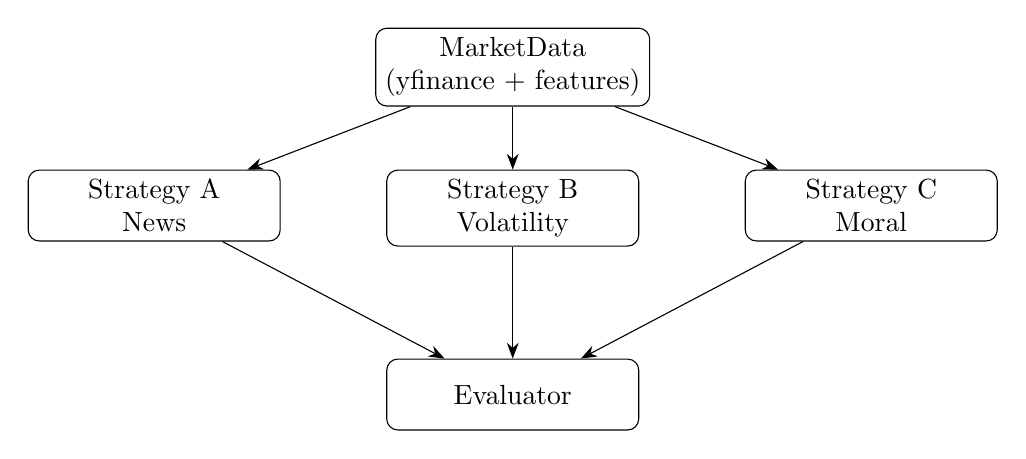
\begin{tikzpicture}[
  node distance=8mm and 12mm,
  box/.style={draw, rounded corners, align=center, minimum width=3.2cm, minimum height=0.9cm},
  arr/.style={-{Stealth[length=2mm]}}
]
\node[box] (md) {MarketData\\(yfinance + features)};
\node[box, below left=of md] (a) {Strategy A\\News};
\node[box, below=of md] (b) {Strategy B\\Volatility};
\node[box, below right=of md] (c) {Strategy C\\Moral};
\node[box, below=3.2cm of md] (ev) {Evaluator};
\draw[arr] (md) -- (a);
\draw[arr] (md) -- (b);
\draw[arr] (md) -- (c);
\draw[arr] (a) -- (ev);
\draw[arr] (b) -- (ev);
\draw[arr] (c) -- (ev);
\end{tikzpicture}
\end{center}

\section{Stock Selection and Rationale}

Table~\ref{tab:stocks} lists four U.S.\ equities chosen to span different regimes: large-cap growth/momentum proxy (NVDA), high-beta volatile name (TSLA), defensive healthcare (JNJ), and stable consumer staple (KO).

\begin{table}[h]
  \centering
  \begin{tabular}{@{}ll@{}}
    \toprule
    Ticker & Intended regime \\
    \midrule
    NVDA & Large-cap, high attention, tech beta \\
    TSLA & Volatile / momentum-sensitive \\
    JNJ & Defensive, lower drama \\
    KO & Staple, typically lower realized vol \\
    \bottomrule
  \end{tabular}
  \caption{Stock selection intent (qualitative).}
  \label{tab:stocks}
\end{table}

\section{Results by Stock}

Table~\ref{tab:results} summarizes graded strategies A/B and extension C from \texttt{outputs/summary.json}. Confidence values come from each ticker file.

\begin{table}[h]
  \centering
  \footnotesize
  \begin{tabular}{@{}lccccccc@{}}
    \toprule
    Ticker & A (News) & Conf. & B (Vol.) & Conf. & C (Moral) & Conf. & Spread \\
    \midrule
    NVDA & HOLD & 6 & HOLD & 6 & HOLD & 6 & 0 \\
    TSLA & HOLD & 8 & HOLD & 8 & HOLD & 6 & 2 \\
    JNJ  & HOLD & 6 & HOLD & 6 & HOLD & 6 & 0 \\
    KO   & HOLD & 6 & HOLD & 8 & HOLD & 6 & 2 \\
    \bottomrule
  \end{tabular}
  \caption{Decisions and confidence (1--10) for the 2026-04-11 live run (with Alpha Vantage on NVDA/JNJ/KO; TSLA throttled). Spread is max minus min confidence across A/B/C.}
  \label{tab:results}
\end{table}

\subsection{Direct excerpts from JSON outputs}

\textbf{NVDA (News Sentiment Follower, with live news):} \emph{``Recent news articles exhibit mixed sentiment\ldots\ the overall market data suggests a steady upward trend, with NVDA's current price at \$188.63 and a 30-day percentage change of 1.4\%. The average daily volume is substantial\ldots\ I lean towards HOLD unless extreme price action contradicts this analysis.''}

\textbf{TSLA (News Sentiment Follower, empty feed after throttle):} \emph{``No recent news available (articles\_count = 0) and avg\_sentiment\_score is null. Current price (\$348.95) is near the moving average (370.85). Volatility (0.023797) is low\ldots\ The recent drop (-14.44\%) may be a buying opportunity.''} (Note: \texttt{news\_features.note} records Alpha Vantage's request to slow free-tier calls---not a missing key.)

\textbf{JNJ (Volatility Averse, with sentiment in payload):} \emph{``Standardized volatility metrics indicate low turbulence (std\_daily\_return\_90d = 0.010491, atr\_14 = 4.2214)\ldots\ The overall sentiment score from news articles suggests a moderate positive tone (avg\_sentiment\_score = 0.10895274999999997)\ldots''}

\subsection{Evaluator}
Across tickers, the evaluator still records \textbf{unanimous HOLD} but the \texttt{pattern\_note} field differentiates emphasis when present---e.g.\ NVDA flags Moral Trader's focus on headline language and valuation risk versus A/B on mixed sentiment and moderate vol metrics; TSLA notes the large 30-day drawdown as an outlier theme despite agreement on HOLD.

\section{Patterns of Agreement and Disagreement}

\textbf{Observed pattern in this run: broad agreement.} For all four tickers, strategies A/B/C agreed on \textbf{HOLD}, yielding \texttt{total\_agreements = 4} and \texttt{total\_disagreements = 0} in \texttt{outputs/summary.json}.

\textbf{Interpretation (not just restatement).} Agreement persists for different reasons than in the ``no API key'' regime:
\begin{itemize}
  \item \textbf{Partial news coverage:} NVDA, JNJ, and KO carry 20 articles and numeric \texttt{avg\_sentiment\_score}, yet Strategy~A still outputs HOLD when sentiment is \emph{mixed} or only weakly directional relative to price. TSLA's feed is empty on this run because Alpha Vantage returned a \textbf{rate-limit / pacing} message after earlier calls in the same batch---Strategy~A then behaves like the old no-news fallback (price and vol language only).
  \item \textbf{HOLD despite heterogeneous tape:} TSLA's 30-day return is $-14.44\%$ while NVDA is slightly up and JNJ/KO are comparatively quiet; all three strategies still output HOLD---models emphasize bounded realized volatility and conservative interpretation of sentiment scores rather than aggressive directional bets.
\end{itemize}

\textbf{Confidence spread (quantitative nuance).} A spread of 2 appears on \textbf{TSLA} (Moral Trader at 6 vs.\ both graded agents at 8) and on \textbf{KO} (Volatility Averse at 8 vs.\ News and Moral at 6). \textbf{NVDA} and \textbf{JNJ} show identical triples (all 6).

\textbf{Where sharper disagreement would likely appear.} Spacing Alpha Vantage calls (\texttt{ALPHAVANTAGE\_MIN\_INTERVAL\_SEC}) so TSLA also gets a feed; choosing tickers or windows where \texttt{avg\_sentiment\_score} is strongly positive/negative while realized vol is elevated would stress-test News vs.\ Volatility philosophies.

\section{Failure or Surprise Case}

\textbf{Surprise 1 (behavioral):} even with \textbf{live news} on NVDA/JNJ/KO (20 articles, non-null \texttt{avg\_sentiment\_score}), all agents still choose \textbf{HOLD} on every ticker---including TSLA where the tape is sharply negative over 30 days but Strategy~B still frames turbulence as ``acceptable'' for a HOLD.

\textbf{Surprise 2 (operational):} \textbf{TSLA} received \textbf{no articles} in the same run because Alpha Vantage's free tier asked to space requests; the JSON stores that explanation in \texttt{news\_features.note}. That reintroduces an \emph{asymmetric information} condition across tickers in one batch.

\textbf{Surprise 3 (model quality):} on KO, Moral Trader's justification claims sentiment is ``slightly negative'' while \texttt{avg\_sentiment\_score} is \textbf{positive} ($\approx 0.248$)---an internal inconsistency worth documenting under responsible AI use.

\textbf{Mitigation:} set \texttt{ALPHAVANTAGE\_MIN\_INTERVAL\_SEC} (e.g.\ 1--15) between ticker calls; rerun TSLA after a pause; tighten prompts against contradicting numeric fields; consider a second pass only for tickers that returned empty feeds.

\section{Reflection}

If I had to follow \textbf{one graded strategy for one month with \$10{,}000}, I would still lean \textbf{Volatility Averse} for \textbf{operational robustness}: when Alpha Vantage throttles or returns an empty feed, Strategy~A partially collapses to the same price/vol heuristics, while Strategy~B is designed around measurable turbulence. For tickers where news is \textbf{reliably} populated (NVDA/JNJ/KO here), I would revisit whether Strategy~A's mixed-sentiment HOLD is too conservative---that is a fair month-long experiment with the News follower \emph{if} API pacing is fixed.

A \textbf{hybrid} would gate sentiment: only allow Strategy A to override when $\lvert\texttt{avg\_sentiment\_score}\rvert$ exceeds a threshold \emph{and} \texttt{articles\_count} is above a floor; otherwise defer to Strategy B's risk checks; \textbf{skip} sentiment overrides when \texttt{news\_features.note} indicates throttle or error.

\appendix
\section*{Bonus artifact: backtest snapshot}
The repository includes \texttt{outputs/backtest.json} (deterministic heuristic proxy; not identical to live LLM decisions). For the run committed alongside the 2026-04-11 outputs, \texttt{overall\_winner} is \textbf{news\_sentiment\_heuristic} (26 weeks, 20-day forward return scoring).

Per-ticker heuristic hit rates (news vs.\ volatility) and winner flags:
\begin{table}[h]
  \centering
  \footnotesize
  \begin{tabular}{@{}lccc@{}}
    \toprule
    Ticker & News hit & Vol.\ hit & Heuristic winner \\
    \midrule
    NVDA & 0.3043 & 0.3913 & volatility\_averse \\
    TSLA & 0.4348 & 0.4348 & tie \\
    JNJ  & 0.4348 & 0.1739 & news\_sentiment \\
    KO   & 0.3043 & 0.3043 & tie \\
    \bottomrule
  \end{tabular}
  \caption{From \texttt{outputs/backtest.json} \texttt{per\_ticker} (method: \texttt{deterministic\_heuristic\_vs\_forward\_return}).}
\end{table}

\noindent\textbf{Contrast with live agents.} The backtest's point-in-time heuristics disagree frequently in the historical rows (e.g., mixed BUY/SELL vs.\ HOLD signals in \texttt{rows}), while the live 2026-04-11 LLM pass is unanimous HOLD on the \emph{current} snapshot---a useful honesty point for grading: the bonus artifact measures a different object than the conversational strategies on ``today's'' JSON.

\end{document}
